\documentclass{article}

\usepackage[utf8]{inputenc}

\usepackage{amsmath, bm}
\usepackage{graphicx}
\usepackage{amssymb}
\usepackage{float}
\usepackage{caption}
\usepackage{subcaption}
\usepackage{hyperref}
\usepackage{tikz}
\usepackage{pgfgantt}
\usepackage{layout}

\usepackage[margin=1in]{geometry}
\usepackage{listings}
\usepackage{xcolor}
\usepackage{color, colortbl}
\usepackage{textgreek}
\usepackage{mathrsfs}
\usepackage{savetrees}

\usepackage[siunitx]{circuitikz}
\usetikzlibrary{shapes.geometric}

\usetikzlibrary{calc}
\usetikzlibrary{angles,quotes} % for pic
\usetikzlibrary{patterns,snakes}
\usetikzlibrary{arrows}
\usetikzlibrary{shapes.geometric, arrows}
\tikzset{>=latex} % for LaTeX arrow head

\setlength{\parskip}{\baselineskip}%
\setlength{\parindent}{0pt}%
\linespread{0.9}


\definecolor{codegreen}{rgb}{0,0.6,0}
\definecolor{codegray}{rgb}{0.5,0.5,0.5}
\definecolor{codepurple}{rgb}{0.58,0,0.82}
\definecolor{backcolour}{rgb}{0.95,0.95,0.92}

\lstdefinestyle{mystyle}{
    backgroundcolor=\color{backcolour},   
    commentstyle=\color{codegreen},
    keywordstyle=\color{magenta},
    numberstyle=\tiny\color{codegray},
    stringstyle=\color{codepurple},
    basicstyle=\ttfamily\footnotesize,
    breakatwhitespace=false,         
    breaklines=true,                 
    captionpos=b,                    
    keepspaces=true,                 
    numbers=left,                    
    numbersep=5pt,                  
    showspaces=false,                
    showstringspaces=false,
    showtabs=false,                  
    tabsize=2
}
\tikzset{
    cg/.style={
        draw,
        circle,
        thick,
        minimum size=0.2cm, % Adjust the size of the circle
        inner sep=0,      % Remove extra padding
        append after command={
            \pgfextra{
                \draw[thick] (\tikzlastnode.south) -- (\tikzlastnode.north);
                \draw[thick] (\tikzlastnode.west) -- (\tikzlastnode.east);
            }
        }
    }
}
\newcommand\textganttbar[4]{%
    \ganttbar{#1}{#3}{#4}
    \ganttbar[inline,bar label font=\footnotesize]
    {#2}{#3}{#4}
}
\newcommand\textganttmilestone[3]{%
    \ganttmilestone{#1}{#3}
    \ganttmilestone[inline,bar label font=\footnotesize]
    {#2}{#3}
}

\tikzset{
    pics/microph/.style={code={ 
        \draw[black, line width=.2em, rounded corners=1.7ex] 
            (-.85em,4.5ex) -- (-.85em,2ex) -- (.85em,2ex) -- (.85em,4.5ex);
        \fill[black] 
            (-.6em,5ex) to[rounded corners=1.2ex]  
            (-.6em,2.5ex) to[rounded corners=1.2ex] (.6em,2.5ex)
            -- (.6em,5ex) to[rounded corners=.2ex] ++(-.85em,0) to[rounded corners=.2ex] ++(0,.35ex) -- ++(.85em,0)  
            -- (.6em,5.5ex) to[rounded corners=.2ex] ++(-.85em,0) to[rounded corners=.2ex] ++(0,.35ex) -- ++(.85em,0)
            -- (.6em,6ex) to[rounded corners=.2ex] ++(-.85em,0) to[rounded corners=.2ex] ++(0,.35ex) -- ++(.85em,0)
            -- (.6em,6.5ex) to[rounded corners=.2ex] ++(-.85em,0) to[rounded corners=.2ex] ++(0,.35ex) -- ++(.85em,0)
            to[rounded corners=1.2ex]
            (.6em,8ex) to[rounded corners=1.2ex]
            (-.6em,8ex) to cycle; 
        \fill[black] (-.1em,1.8ex) rectangle (.1em,.5ex);
        \fill[black] (-.5em,.5ex) rectangle (.5em,0);
    }},
}

\lstset{style=mystyle}

\tikzstyle{startstop} = [rectangle, rounded corners, minimum width=3cm, minimum height=1cm,text centered, draw=black, fill=red!30]
\tikzstyle{process} = [rectangle, minimum width=3cm, minimum height=1cm, text centered, draw=black, fill=orange!30]
\tikzstyle{decision} = [diamond, minimum width=3cm, minimum height=1cm, text centered, draw=black, fill=green!30]
\tikzstyle{io} = [trapezium, trapezium left angle=70, trapezium right angle=110, minimum width=3cm, minimum height=1cm, text centered, draw=black, fill=blue!30]
\tikzstyle{arrow} = [thick,->,>=stealth]

\begin{document}
\immediate\write18{py mergebib.py}

\title{Acoustic Signatures of Quadcopter Propellers}
\author{Louis Pender LWP26}
\date{Janurary 2025}
\maketitle 

\begin{center}
    \textbf{Summary}

    The motivation for studying harmonic noise reduction of propellers is discussed, highlighting the potential of looped propeller designs to address noise concerns in drone applications.
    Mechanisms of tonal noise reduction, including blade sweep and uneven blade spacing, are reviewed with a focus on their relevance to looped propellers.
    A theoretical framework, based on Hanson's helicoidal surface theory, is presented alongside Blade Element Momentum (BEM) theory to predict harmonic noise of an arbitrary design.
    Progress on software development, experimental setup, and propeller design is outlined.
    Future work includes implementing BEM, validating results, designing test propellers, and improving theoretical predictions to align with experimental data
\end{center}

%-----------------------------------------------------------------------------------------
\section{Motivation}
%-----------------------------------------------------------------------------------------
Drone based services are becoming increasingly popular in various industries such as agriculture and delivery services.
The adoption of drone services has been limited by public perception and legislation.
A key factor influencing public perception is the noise generated by drones, which is often perceived as intrusive and annoying.
Propulsive efficiency is also important for feasibility as it directly affects flight time and payload capacity.

Recent work has explored innovative methods for reducing noise without compromising performance.
One such propeller design, commonly referred to as toroidal, features looped blades and is known in marine applications.
These have been shown experimentally to reduce Overall Sound Pressure Level (OASPL) and Psychoacoustic Annoyance (PA) factors \cite{shima_toroidal}, \cite{ijerph20031955}.
Such PA factors indicate noise at discrete frequencies, or tones, to be a major source of annoyance in propeller noise \cite{ijerph20031955}. %using an extension of Zwicker's psychoacoustic model \cite{DI2016164}.

Mechanisms for tonal noise reduction of standard propellers through sweep and uneven blade spacing are well understood \cite{hanson_influence}, \cite{DOBRZYNSKI1993123}, \cite{doi:10.2514/3.22938}.
However this acoustic theory has not been applied to looped designs, which feature unevenly spaced and highly swept blades.
Looped propellers structure also allows for larger sweep than standard propellers \cite{shima_toroidal}
A fast method to predict the tonal noise would enable iterative design methods to optimise the looped propeller design for noise reduction.

\section{Project Management}

Objectives for the project are classified into groups: Acoustic and aerodynamic theory, and also their respective practical setups. 
A seperate group is made for progress on the software tool.
The key component of the project is the prediction of harmonic noise for an arbitrary propeller design.
Hanson's method \cite{hanson_theory}, described in detail later, requires knowledge of aerodynamic forces acting over the blade.
These are calculated in the most reduced represenation of the problem for arbitrary designs using Blade Element Momentum (BEM) theory, also discussed later.
A key point of future work includes improvements to the implementation of BEM theory to better match the results.
% organise report structure 
% require far field noise
% 
\begin{figure}[H]
    \centering
    \resizebox{\textwidth}{!}{
    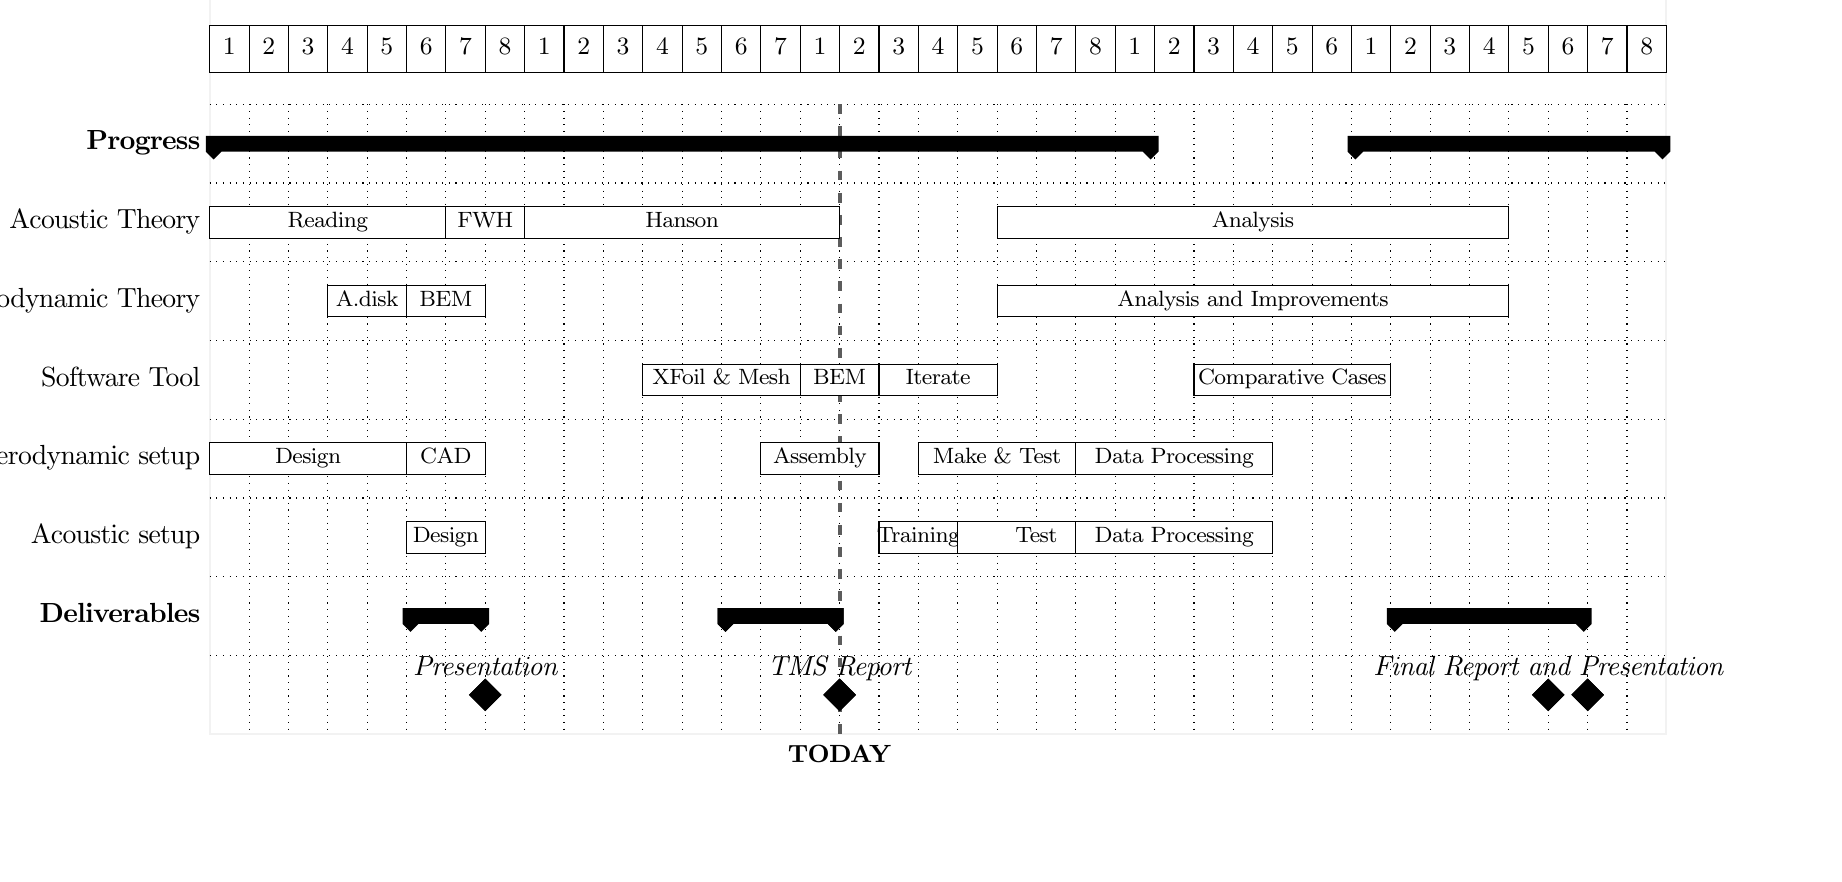
\begin{tikzpicture}[x=.5cm, y=1cm]
    \begin{ganttchart}[
        canvas/.append style={fill=none, draw=black!5, line width=.75pt},
        vgrid,
        hgrid,
        %hgrid style/.style={draw=black!5, line width=.75pt},
        %vgrid={*1{draw=black!5, line width=.75pt}},
        today=16,
        today rule/.style={
        draw=black!64,
        dash pattern=on 3.5pt off 4.5pt,
        line width=1.5pt,
        link/.style={-latex, line width=1.5pt},
        },
        today label font=\small\bfseries]{1}{37}
        \gantttitle{Michaelmas Term}{8} \gantttitle{Christmas Break}{7} \gantttitle{Lent Term}{8} \gantttitle{Easter Break}{6} \gantttitle{Easter Term}{8}\\
        \gantttitlelist{1,...,8}{1} \gantttitlelist{1,...,7}{1} \gantttitlelist{1,...,8}{1} \gantttitlelist{1,...,6}{1} \gantttitlelist{1,...,8}{1}\\
        \ganttgroup{Progress}{1}{24} \ganttgroup{}{30}{37}\\
        \textganttbar{Acoustic Theory}{Reading}{1}{6} \textganttbar{}{FWH}{7}{8} \textganttbar{}{Hanson}{9}{16} \textganttbar{}{Analysis}{21}{33} \\
        \textganttbar{Aerodynamic Theory}{A.disk}{4}{5} \textganttbar{}{BEM}{6}{7} \textganttbar{}{Analysis and Improvements}{21}{33}\\
        \textganttbar{Software Tool}{XFoil \& Mesh}{12}{15}\textganttbar{}{BEM}{16}{17} \textganttbar{}{Iterate}{18}{20} \textganttbar{}{Comparative Cases}{26}{30}\\
        \textganttbar{Aerodynamic setup}{Design}{1}{5} \textganttbar{}{CAD}{6}{7} \textganttbar{}{Assembly}{15}{17} \textganttbar{}{Make \& Test}{19}{22} \textganttbar{}{Data Processing}{23}{27} \\
        \textganttbar{Acoustic setup}{Design}{6}{7}\textganttbar{}{Training}{18}{19} \textganttbar{}{Test}{20}{23} \textganttbar{}{Data Processing}{23}{27}\\
        %\ganttlink{elem2}{elem3}
        %\ganttlink{elem3}{elem4}

        \ganttgroup{Deliverables}{6}{7} \ganttgroup{}{14}{16} \ganttgroup{}{14}{16} \ganttgroup{}{31}{35} \\

        \textganttmilestone{}{Presentation}{7} \textganttmilestone{}{TMS Report}{16} \textganttmilestone{}{Final Report and Presentation}{34} \textganttmilestone{}{}{35}
    \end{ganttchart}
    \end{tikzpicture}
    }
    \caption{Gantt chart of project timeline}
    \label{fig:gantt}
\end{figure}

\begin{table}[H]
    \centering
    \resizebox{\textwidth}{!}{
    \begin{tabular}{|p{4cm}|p{4cm}|p{5cm}|p{5cm}|}
    \hline
    \textbf{Risk} & \textbf{Consequence} & \textbf{Mitigation} & \textbf{Contingency} \\ \hline
    Discrepancy between aerodynamic and acoustic tests. & Results may not align, reducing reliability of findings. & Compare noise of uninsulated acoustic setup with aerodynamic setup & Identify source and quantify the discrepancy and if required redesign setup. \\ \hline
    Blade deflection. & Lower thrust and efficiency; altered noise characteristics & Limit sweep to $60^\circ$ and select thick airfoil sections. & Increase airfoil thickness or reduce sweep. \\ \hline
    Aeroelastic flutter. & Structural damage, catastrophic failure. & High acceleration to reduce modal responses. Operator not in same room. & Reduce operating point. \\ \hline
    Motor noise interference with acoustic measurements. & Misinterpretation of acoustic signatures. & Acoustic insulation of motor. Measurement of load-matched motor noise. & Spectral subtraction of load-matched signal. \\ \hline
    Motor overheating in acoustic insulation. & Damage to motor; invalid results due to test interruptions & Monitor temperature, pausing to allow cooling & Increase passive cooling with heatsink. \\ \hline
    Large motor currents inducing voltages in strain gauge wires. & Interference with force measurements, leading to inaccurate data. & Time average readings and plot dimensional groups. & Use twisted pair wiring and shielding to reduce interference. \\ \hline
    \end{tabular}
    }
    \caption{Project risk analysis with consequences, mitigations, and contingencies.}
\end{table}

\subsection{Experimental setup}

To validate the theoretical framework, designed propellers will be manufactured and tested both aerodynamically and acoustically.
The acoustic test will be conducted in an anechoic chamber with a small microphone array to capture directivity of harmonic components.
An attempt to isolate the propeller noise from the motor will be made by placing the motor in a foam box.
Background and motor noise will be measured before and after each test series to ensure repeatability.
Mechanical motor noise is primarily due to structural vibrations from forced unsteady radial loads \cite{motor_vibration}.
This means that they occur at the motor frequency multiplied by the number of pole pairs, which for our motor is 7.
The pole pair count being prime means that for blade counts up to 7 there will be no overlap with the aerodynamic harmonics.

For the aerodynamic test, the thrust and torque of the propeller will be measured on a setup.
Strain gauge load cells were chosen for force measurement over null methods for simplicity and the potential to measure dynamic loads.
The propeller will be mounted upside down to prevent the ground effect, and such that the force is in the direction and range of calibration loads.
It will also be at a 45 degree angle such that a graviational mass can calibrate the torque load cell.
Code written for a preliminary setup using a Pi Pico microcontroller to interface with a HX711 load cell amplifier will be reused.

\subsection{Propeller manufacturing}
Propellers will be manufactured on an Objet30 3D printer which has planar accuracy of $30\mu m$ and minimum layer thickness of $28 \mu m$.
The primary advantage of this printer is the gel support material which does not produce rough connection points on overhangs like traditional resin printers.
An early test print of a looped propeller has been done successfully.
The software tool can export STL files and can also thicken the trailing edge to the minimum layer thickness to avoid being culled during slicing.

\section{Technical Milestone Future work}
The software tool must be finalised with the full implementation of BEM.
This performance must, to some extent, be validated against UIUC propeller data \cite{UIUC_database}.
The mesh geometry for the tips of looped propellers also needs to be improved.
Future practical work involves finishing electronics and adapting previously written code to calibrate and read load cells.
Training to use and assistance setting up of acoustic equipment will be carried out in the coming weeks.

To test the hypothesis the following tests are planned.
A propeller with optimised sweep profile to maximise destructive interference for a chosen harmonic and observer position.
Four seperate airfoil sections for an unswept propeller design to investigate chordwise destructive interference.
Comparison of single and symmetrical looped blade designs to evaluate superimposed model.

\newpage

\section{Practical log}

\begin{itemize}
    %2025-02-03 - 98b21c7 - setup for load cell reading, allbeit with issues
    %2025-02-04 - 8019066 - moved away from riscV because didnt think it was working with the library. never really found out though went through so many tests that ive lost the will to find out why all that matters is that it works now also comes with a fancy multithreaded serial plotter app that i wrote
    \item Feb 5th Reading multiple load cells is more complicated than one. The sample rate of the HX711 boards was fixed to 10Hz from a grounded pin.
    %2025-02-07 - 2596e28 - attached setup to stand in cad
    %2025-02-07 - 050147c - Merge branch 'master' of https://github.com/lpender3672/propeller-acoustics.git
    %2025-02-07 - 772bccf - python reading data
    %2025-02-07 - 71b4c74 - experiment ui
    %2025-02-07 - 418d7a4 - agile i am
    %2025-02-10 - 579a291 - progress with audio collection
    \item Feb 10th Progress writing the multithreaded data collection app.
    %2025-02-11 - d76721a - reading all the data now at the same time
    %2025-02-11 - 513efac - fixed issues with serial thread and calibration but is working now
    %2025-02-13 - 2226be7 - motor control from collection app is working CAD metal acoustic box
    \item Feb 13th CAD work on the acoustic box and motor mount.
    %2025-02-15 - 204ca00 - motor controller moved to seperate thread and cad work
    %2025-02-16 - 300395d - improvements to data collection and calibration
    %2025-02-16 - 0982371 - saving cal data now
    %2025-02-16 - 7b1712c - its messy but the crazy propeller pyramid is working
    %2025-02-17 - c86524c - wallah. calibration and pyramid data
    %2025-02-22 - 69d8ef7 - new setup and associated data starting to implement prop file with saved file
    %2025-02-24 - 04f4985 - progress with geometry
    %2025-02-26 - f02f577 - insane in the membrane
    %2025-02-26 - 3c9cd1c - no longer using fortran
    %2025-02-27 - 6641653 - the first audio data
    \item Feb 27th Motor control software is working and the first audio data has been collected. Frequency setpoints were not working as expected because they were not multiples of the DAQs internal clock rate and so did not match signal generated tones.
    %2025-02-28 - 1660168 - small improvements
    %2025-02-28 - 0ea2d78 - fixed improvements
    %2025-03-01 - 48e07e2 - so the separate calibration gets merged and then a regression gets done. the influence of torque on the thrust load cell is neglible and so that coefficient is set to 0 to help the regession however the regession still struggles to get the , now 5 coefficients, especially for torque because theres only i think 5 datapoints more datapoints are required and will be obtained on monday the thrust coefficient curve is nice and flat up until the top speed. would like to get higher speed points to reach a limit of the motor
    %2025-03-02 - adffe6e - implemented the swept Hermite tip curve improvements to geometry
    \item March 2nd Implemented the swept Hermite tip curve and improved the geometry.
    %2025-03-02 - fddcdb4 - shifting things around in geometry need to clean up a lot of stuff tomorrow morning then work on 4F2 then work on 4A4 then work on implementing the static BEM and reduced airfoil table
    %2025-03-02 - fac5752 - separated xfoil data and geometry data so they can be different lengths. The resolution of lift/drag data was coupled to the airfoil resolution making high resolution airfoils take forever on xfoil also made xfoil run on separate thread
    %2025-03-03 - e131475 - saving props in stl mm now fixed further xfoil_data problems
    %2025-03-03 - 53cde24 - FM plot but its orders of magnitude lower than expected
    %2025-03-03 - b67f98c - added overhead mic
    %2025-03-04 - 0e2fefa - more audio and also tried doing two seperate calibration regressions which yield similar result need to troubleshoot the data
    %2025-03-04 - 547666d - added rotation direction to software something that probably should have been added sooner
    \item March 4th Improved propeller design software to include generation of clockwise and counterclockwise propellers.
    %2025-03-04 - d3120c1 - changed graphs in supo data was being loaded incorrectly
    %2025-03-04 - 8e3b84a - corrected the scale for the stratasys objet30 software
    \item March 4th Fixed scaling issue to be compatible with the Stratasys Objet30 software.
    %2025-03-05 - cc79d1d - some cad work but i didnt like it
    %2025-03-10 - 10eeaaa - fixed issue in hanson that went under the radar. added harmonic plot removed saving to fortran
    %2025-03-12 - f987348 - modifications to casing to pushfit encoder board and mount the load cell the right way round
    \item March 12th Major redesign of the aerodynamic test setup to measure torque. Ceramic bearings and sensitive 200g load cell.
    \item March 12th Encoder board broken thought ODrive was fried. The 1> MHz clock pin was found to only work with the additional capacitance of an oscilloscope probe. Soldered on a 200pF capacitor to the pin and now it works.
    %2025-03-18 - 4913d3d - lots of data and fixed a few bugs fixed cad of acoustic setup to work with new magnet motor mount
    \item March 18th Shaft extender was sitting on a thread and not concentric. New design sits on motor casing and is shown to be concentric.
    %2025-03-18 - 1f38842 - found that the antivibration foam actually makes it worse
    \item March 18th Comparative testing of vibration isolation foam was found to increase noise levels over rubber foot mounts.
    %2025-03-18 - 6ae7e5b - big shift today. a lot of audio processing done harmonic and radar sound graphs
    %2025-03-19 - 21f9f83 - designs to be made improved tangents of tip geometry
    %2025-03-24 - 9a3a0d3 - added an audio pyramid for investigating the variance of sound with speed its untested though as mark needed the odrive cable to charge his phone also made a quick microphone mount design
    %2025-03-24 - fc8e691 - improved pyramid to include logarithmic values for improved logging of dimensionless groups
    \item March 24th Pyramids made logarithmic, reducing data required and allowing for more higher speed data to be collected within the motors temperature limits.
    %2025-03-24 - 95d9c2e - more props and aero data!
    %2025-03-25 - 7c15c9a - decent morning going to do some audio pyramids at specific locations
    %2025-03-25 - 4c08784 - speed varying audio data for all the props and all microphones in a fixed arrangement
    %2025-03-25 - 669ebee - ive been sleeping on vel ramp rate
    %2025-03-31 - 4b72994 - so my laptop did break and this is me on lucy cavs laptop
    \item April 1st increased acceleration ramp rate for faster settle time and achievable speeds within the motor temperature limits.
    %2025-04-09 - cc732a9 - finally fixed the microphones
    %2025-04-09 - ee99a22 - Merge branch 'master' of https://github.com/lpender3672/propeller-acoustics.git
    \item April 9th Higher voltage battery introduced allowing higher speeds to be achieved.
    %2025-04-09 - 9367747 - higher speed data but probably too fast as motor getting really hot now and the off centered spin is getting worse magnet mount fell off actually Joe is remaking the shaft extender with a better connection May also balance the spin will talk to mechanics lab
    %2025-04-11 - c43327f - a lot of data fro different angles
    %2025-04-11 - a8b9e60 - audio for different 2 more radaii at 6 and 8 blade diameters also lots more aero data up to 16000 and 17000 rpm
    %2025-04-18 - cac95b5 - agile commit wrote a function to build a df from all result files
    %2025-04-19 - 5399bcd - using lookup df to plot microphone radar graph
    %2025-04-21 - 6baa85f - visualised some error bars but it wasnt particularly useful. already knew uncertainty at small torque thrusts and speeds was more significant speed uncertainty is still more than expected though
    %2025-04-21 - 72cc713 - Merge branch 'master' of https://github.com/lpender3672/propeller-acoustics.git
    %2025-04-22 - 4300374 - moved some files around and listened to playback of audio
    %2025-04-23 - 6f989b5 - final props and some code improvements
    %2025-04-25 - 74a279b - cleaned up and using poetry now
    %2025-04-25 - 50c7a37 - automatic linting my old code
    %2025-04-25 - 56ff04c - computer do what your programmed to do
    %2025-05-11 - 04cd64c - lots more result files and draft report files
    %2025-05-11 - b98b9d3 - so theres a lot nonlinearity in the SPL which needs to be thought about. This is worrying and points to bad data but there may be an explaination for it. Either way i had hoped for more coherent data
    %2025-05-12 - e7709ac - SPL hysterisis seems independent of settling time so transient effects can be ruled out.
    %2025-05-13 - 144a669 - final tests for 5045 s15 and s45. low speed testing of the 50loop_s50 which broke halfway through testing at 6bd 45 degrees rest of foxeer toroidal was done
    %2025-05-13 - b756c1c - cleanup, turned app into a package which makes it easier to import throughout the codebase structure for graph plotting and audio routines separate from main routines
    %2025-05-13 - cd98ed0 - issue from an autolint?
    %2025-05-14 - 48458ea - added a duration box to help tony record data for the other acoustic experiment tomorrow
    %2025-05-14 - 5da3bf8 - tomorrow ill clean this up a bit more and move the functions to the right files has been some interesting graphs but ill spend all of tomorrow on it However the radial variation data seems concering The to do list is still to write up practical parts And some meshgrid plotting utilities Potentially the inclusion of integrated harmonics Also to speed the process up i need to save the processed data to a cache
    %2025-05-14 - 31f3dd1 - Merge branch 'master' of https://github.com/lpender3672/propeller-acoustics.git

\end{itemize}

\begin{figure}[H]
    \centering
    \begin{subfigure}[t]{0.32\textwidth}
        \centering
        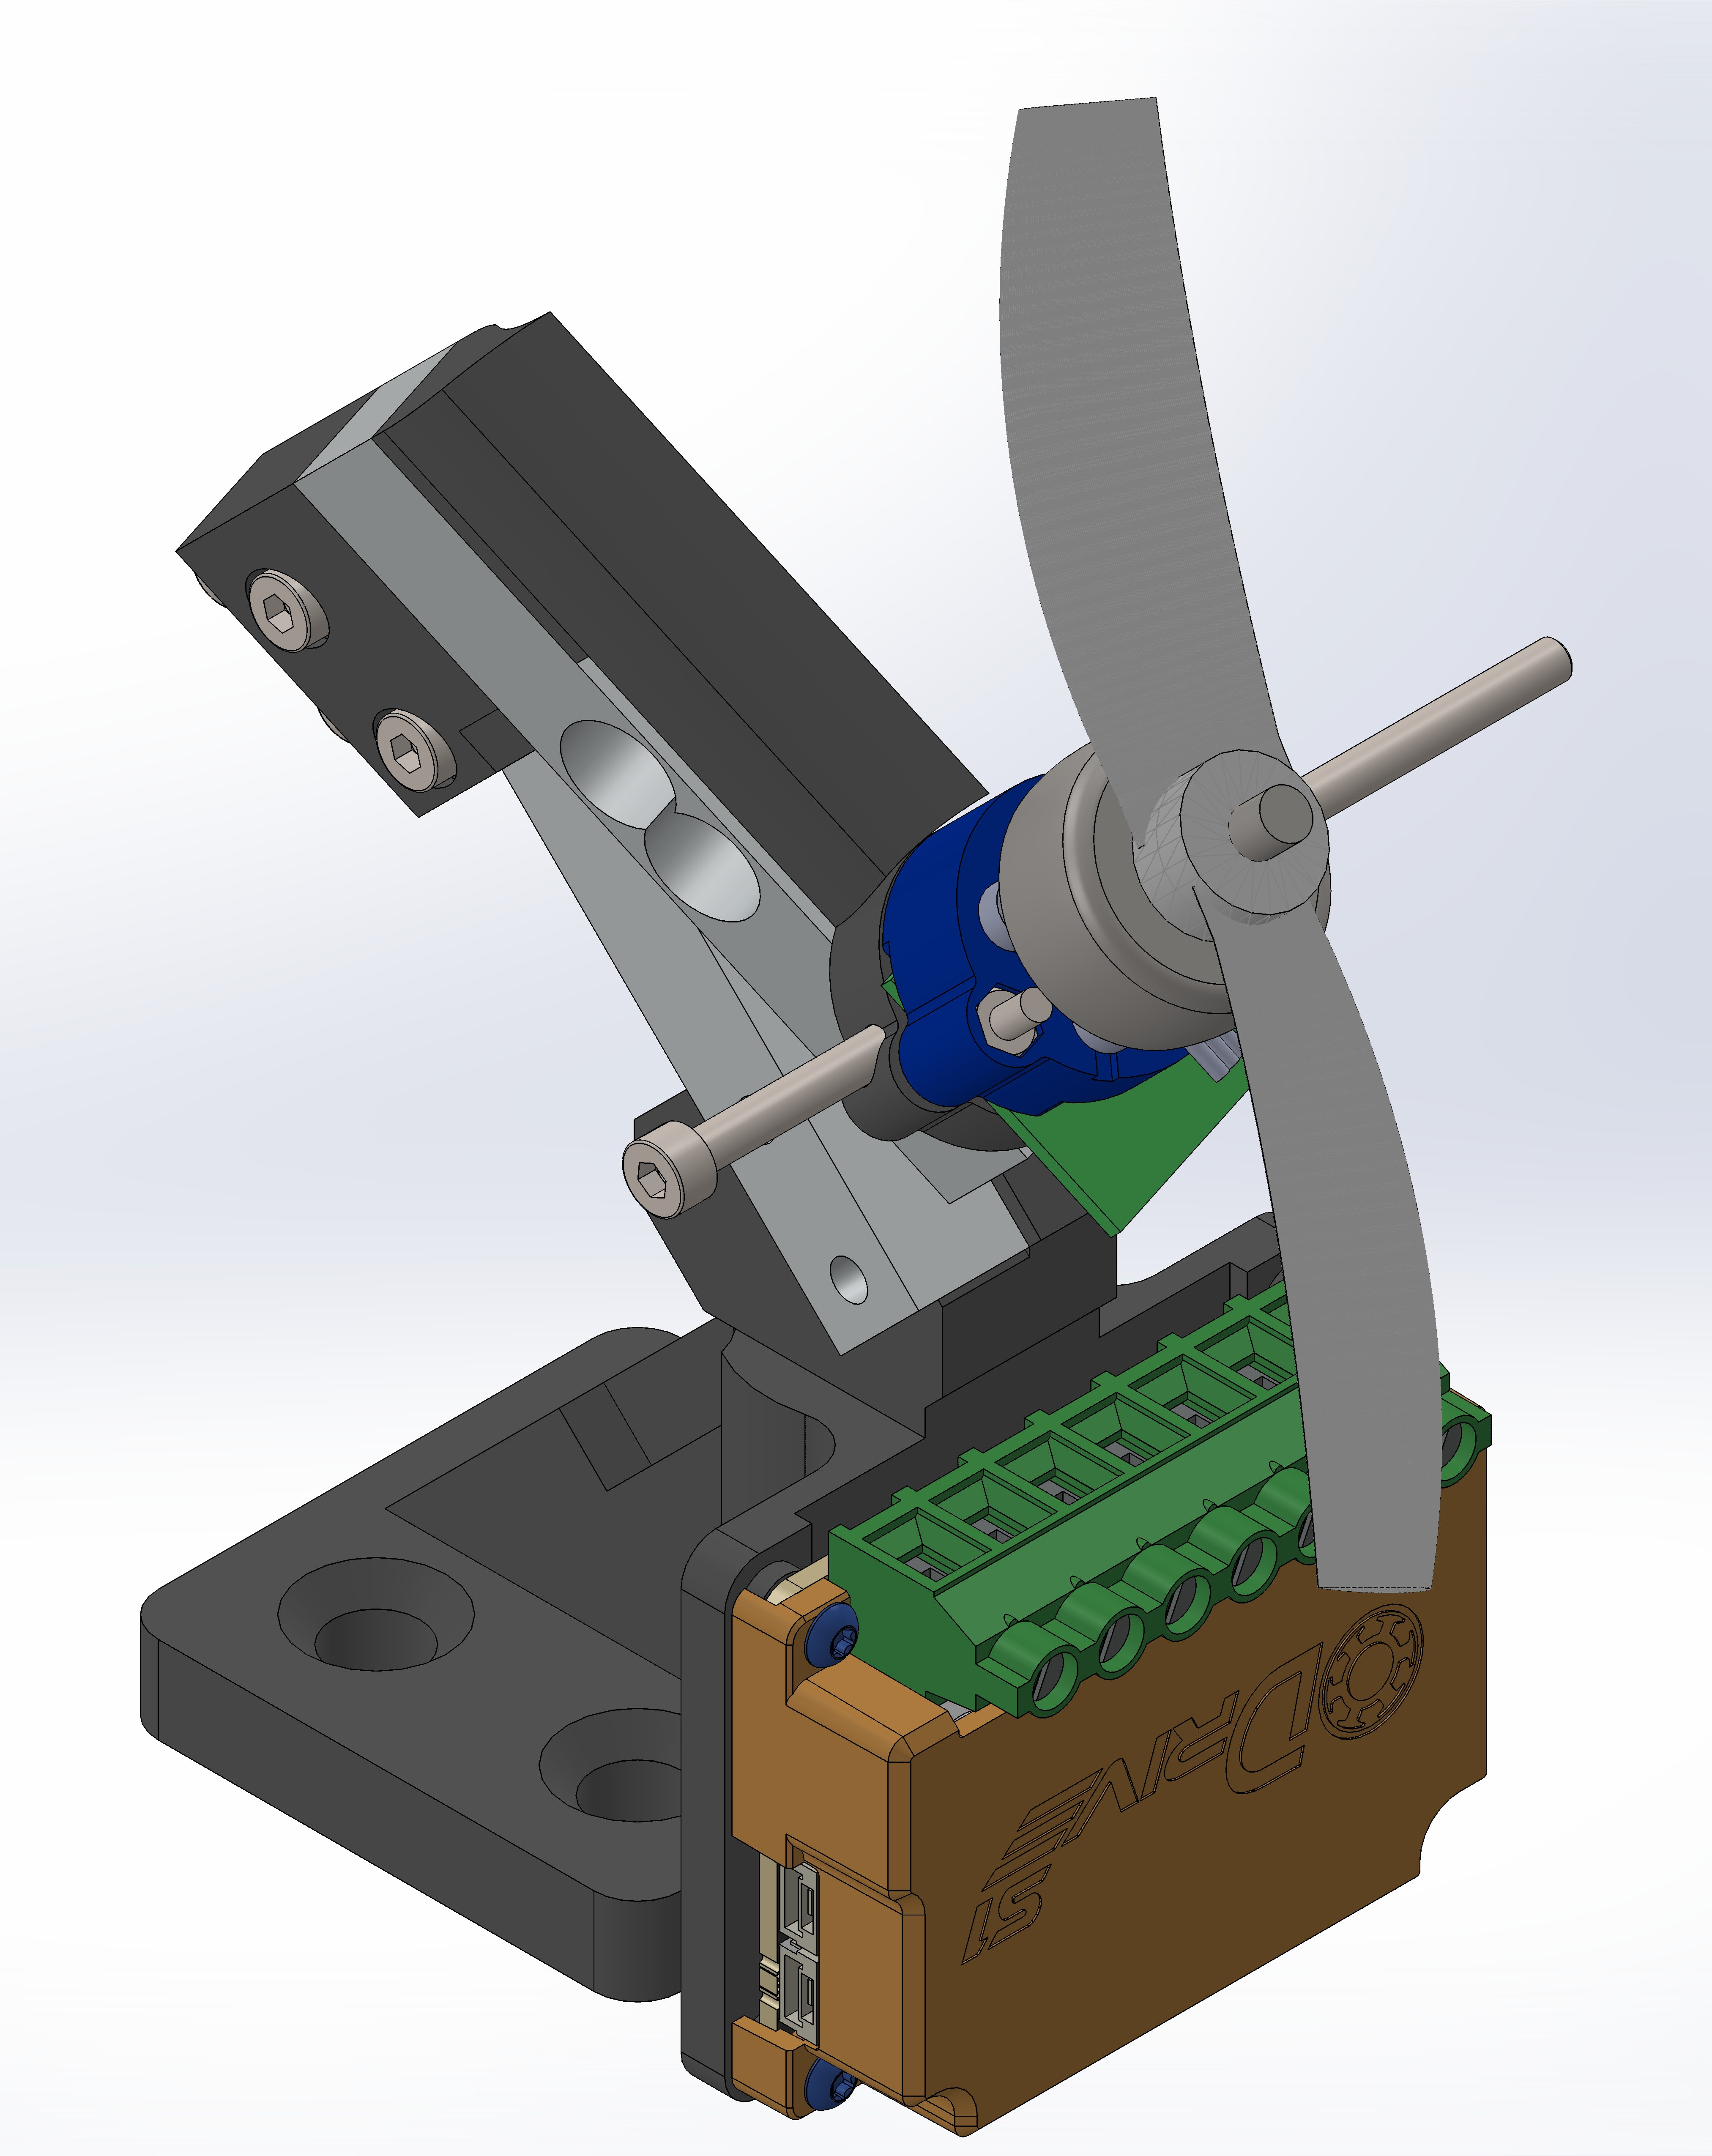
\includegraphics[width=\textwidth]{figures/aero1.JPG}
        \caption{}
        \label{fig:aero1}    
    \end{subfigure}
    \begin{subfigure}[t]{0.32\textwidth}
        \centering
        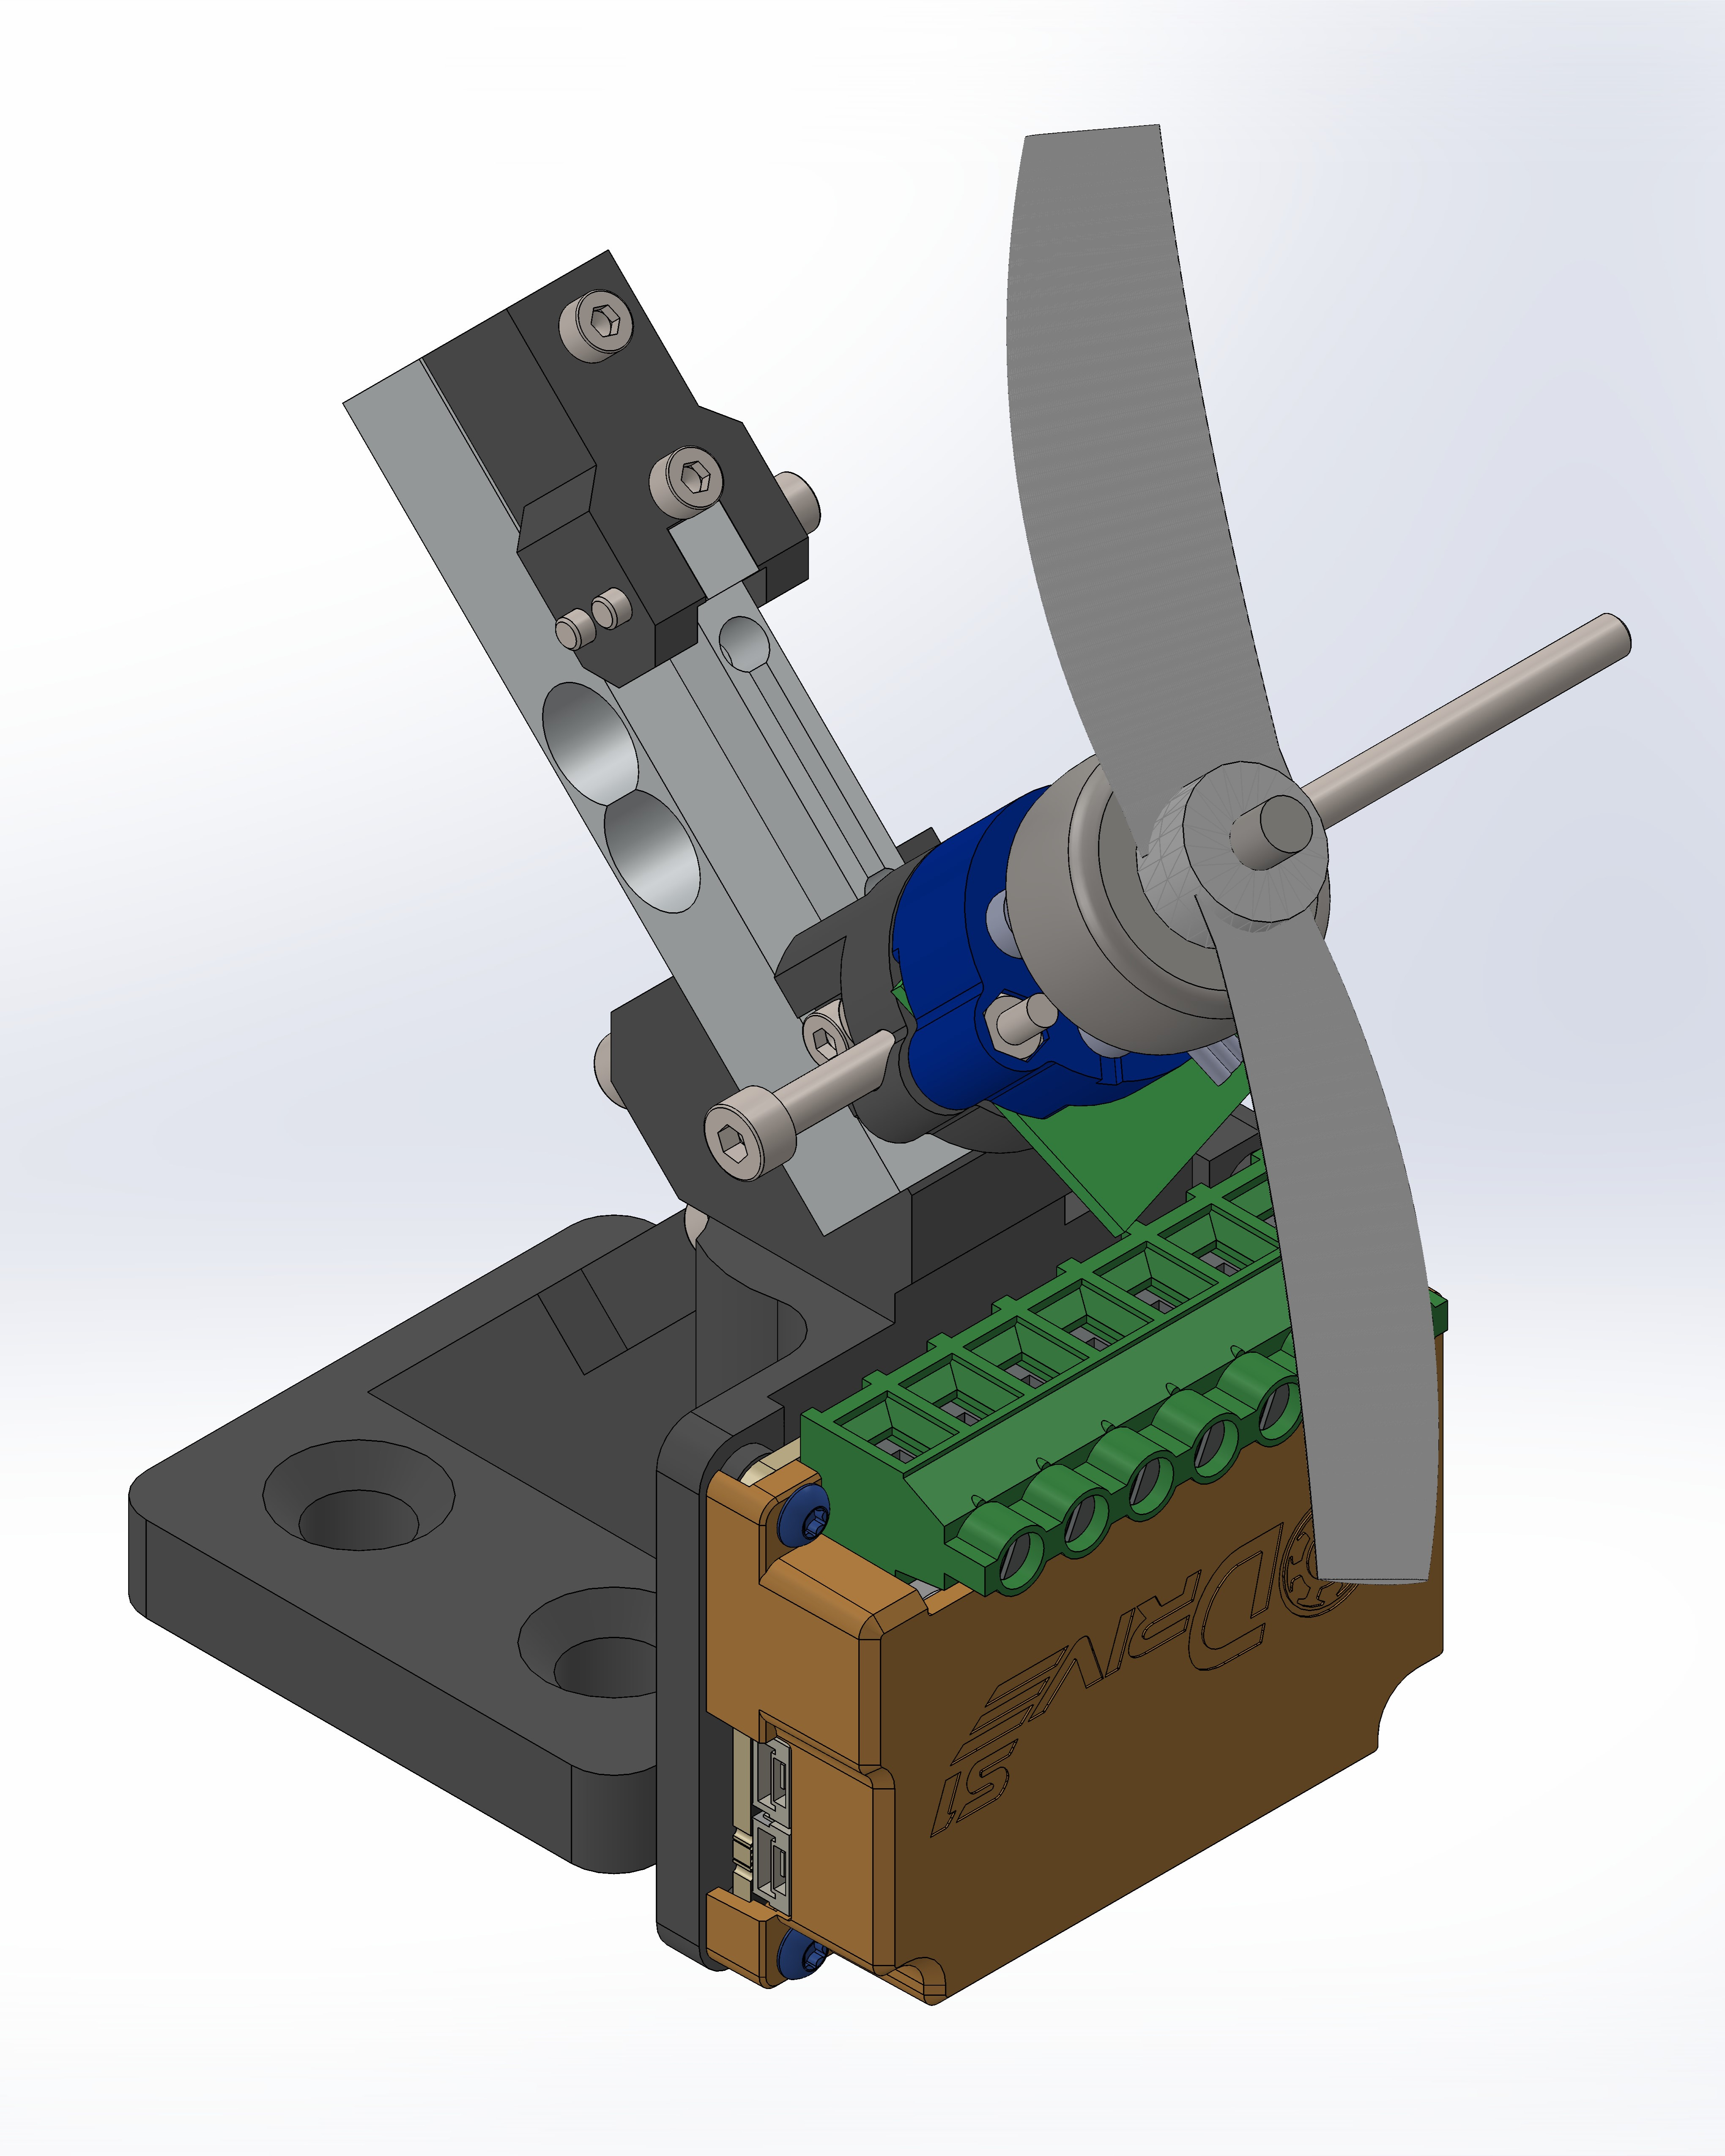
\includegraphics[width=\textwidth]{figures/aero2.JPG}
        \caption{}
        \label{fig:aero2}    
    \end{subfigure}
    \begin{subfigure}[t]{0.32\textwidth}
        \centering
        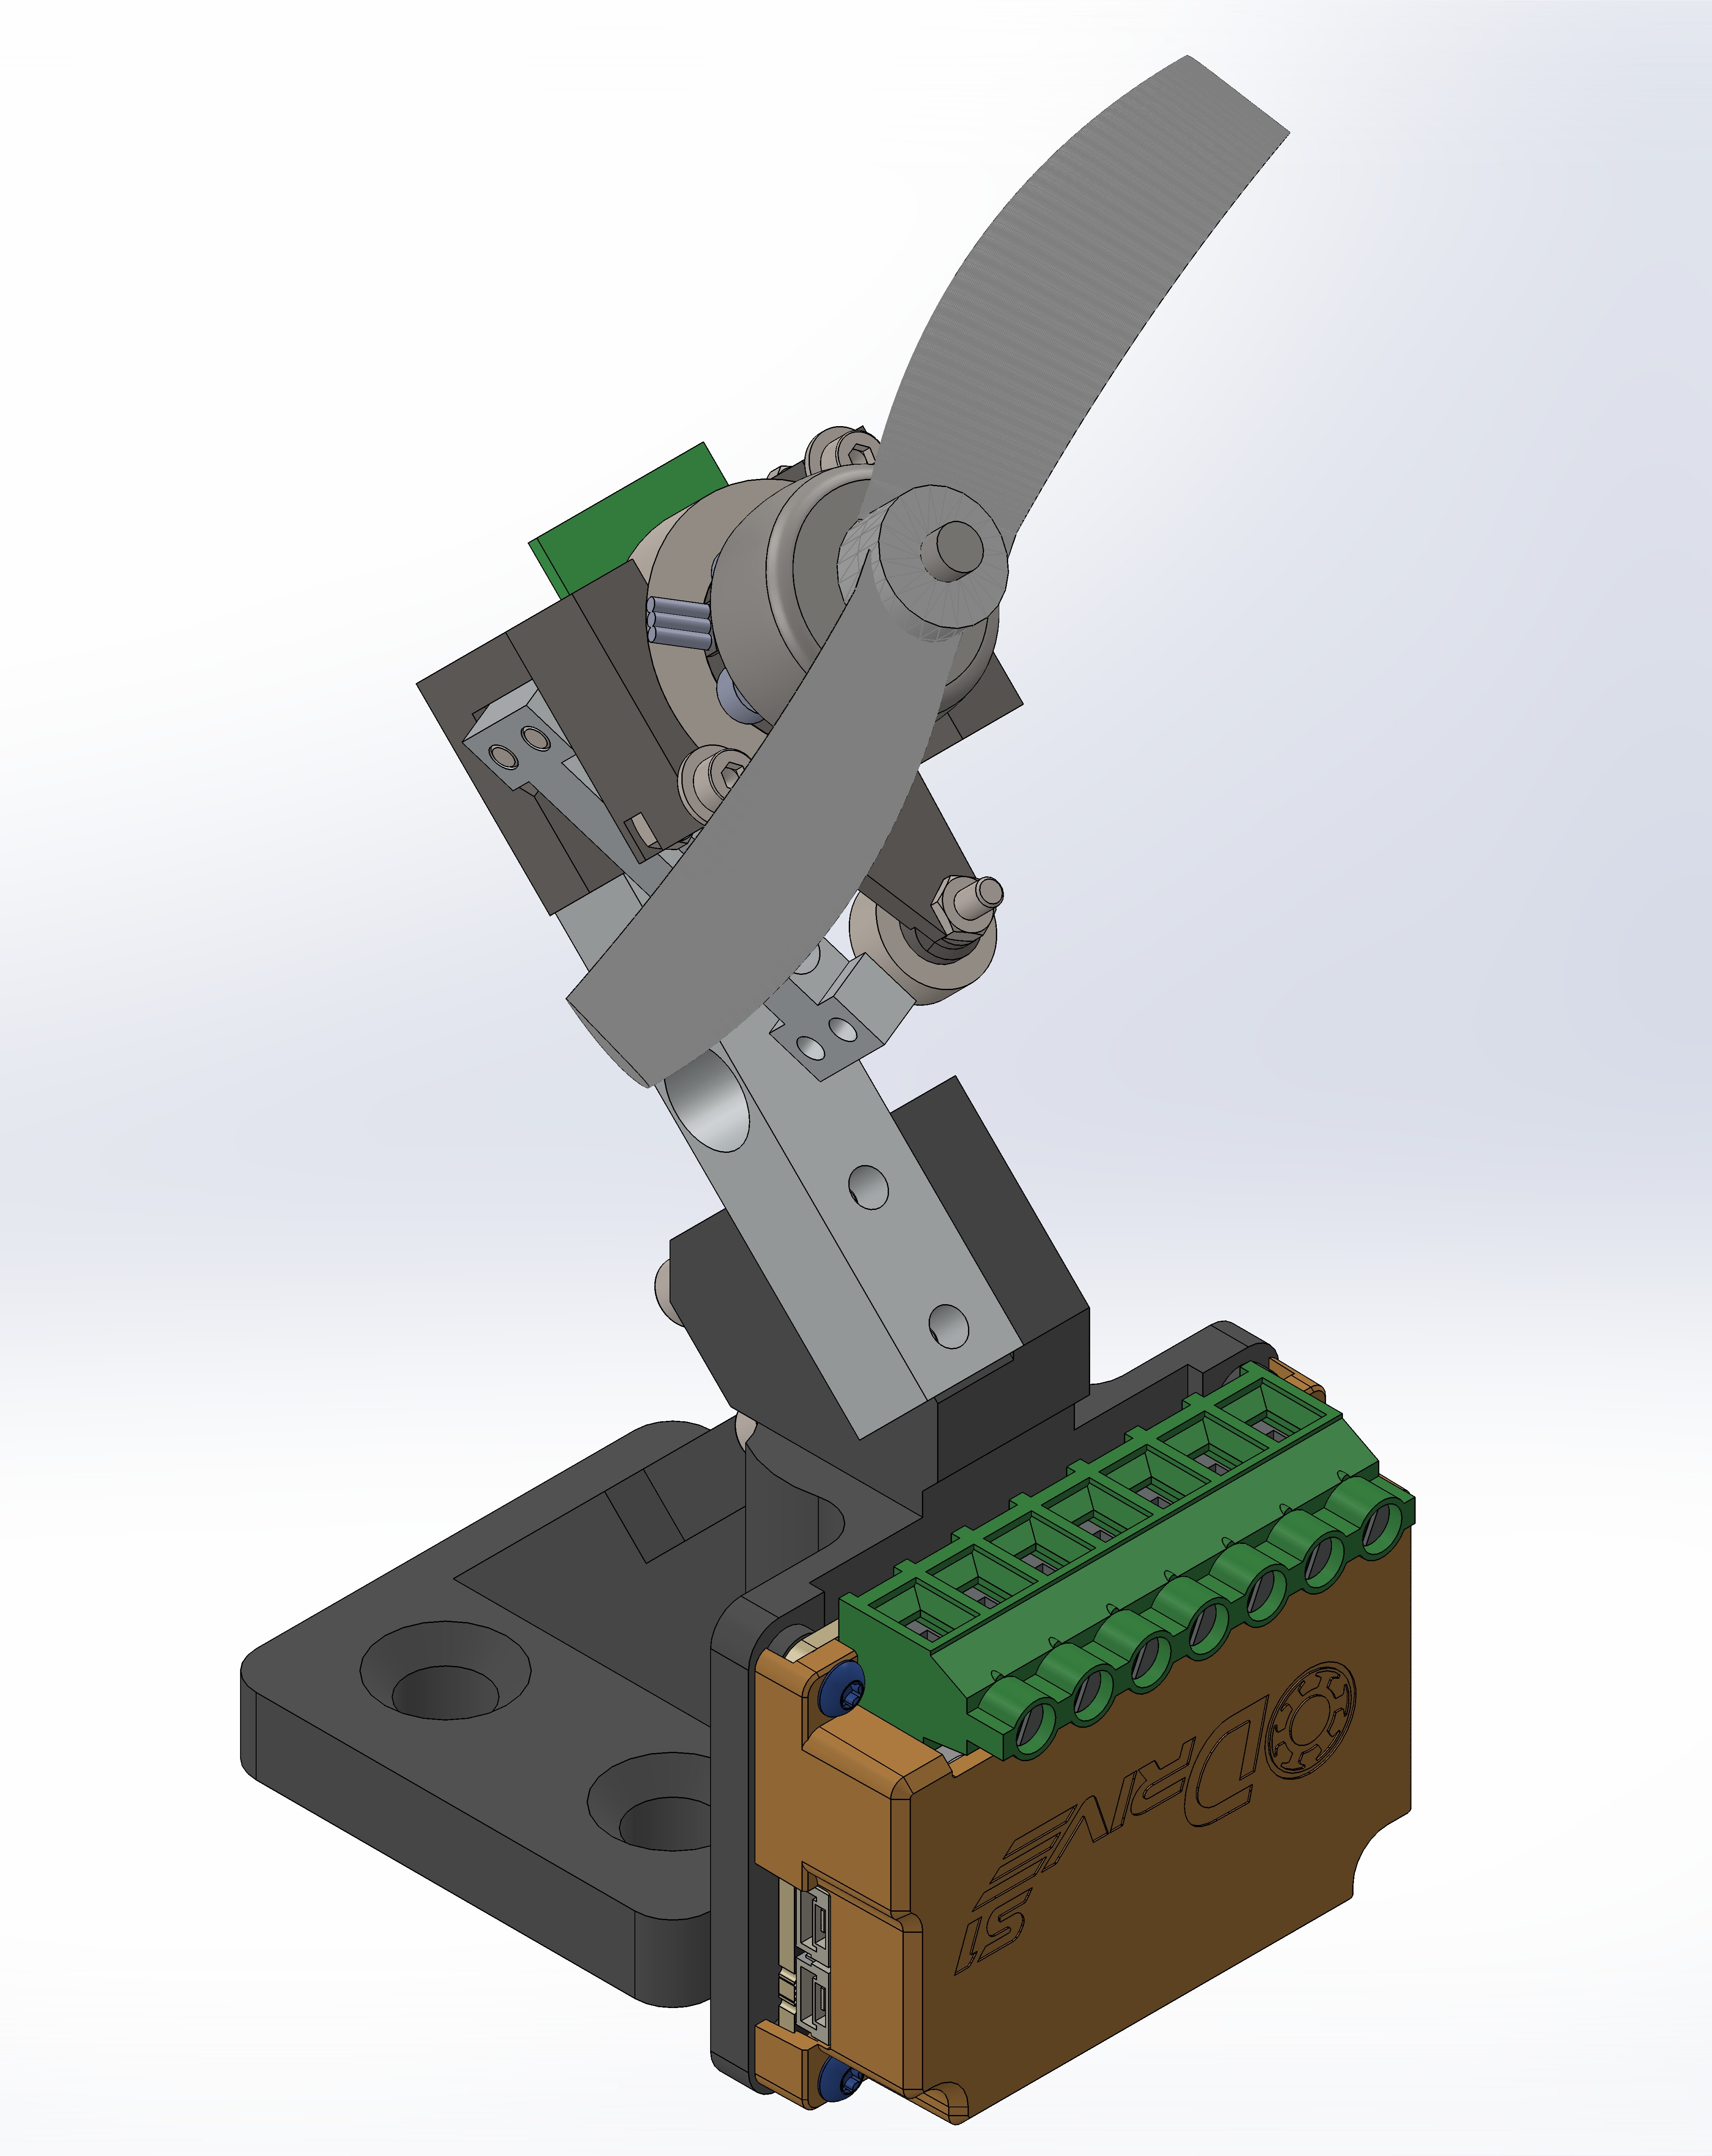
\includegraphics[width=\textwidth]{figures/aero3.JPG}
        \caption{}
        \label{fig:aero3}    
    \end{subfigure}
    \caption{Iterations of the aerodynamic test rig}
\end{figure}

\begin{figure}[H]
    \centering
    \begin{subfigure}[t]{0.30\textwidth}
        \centering
        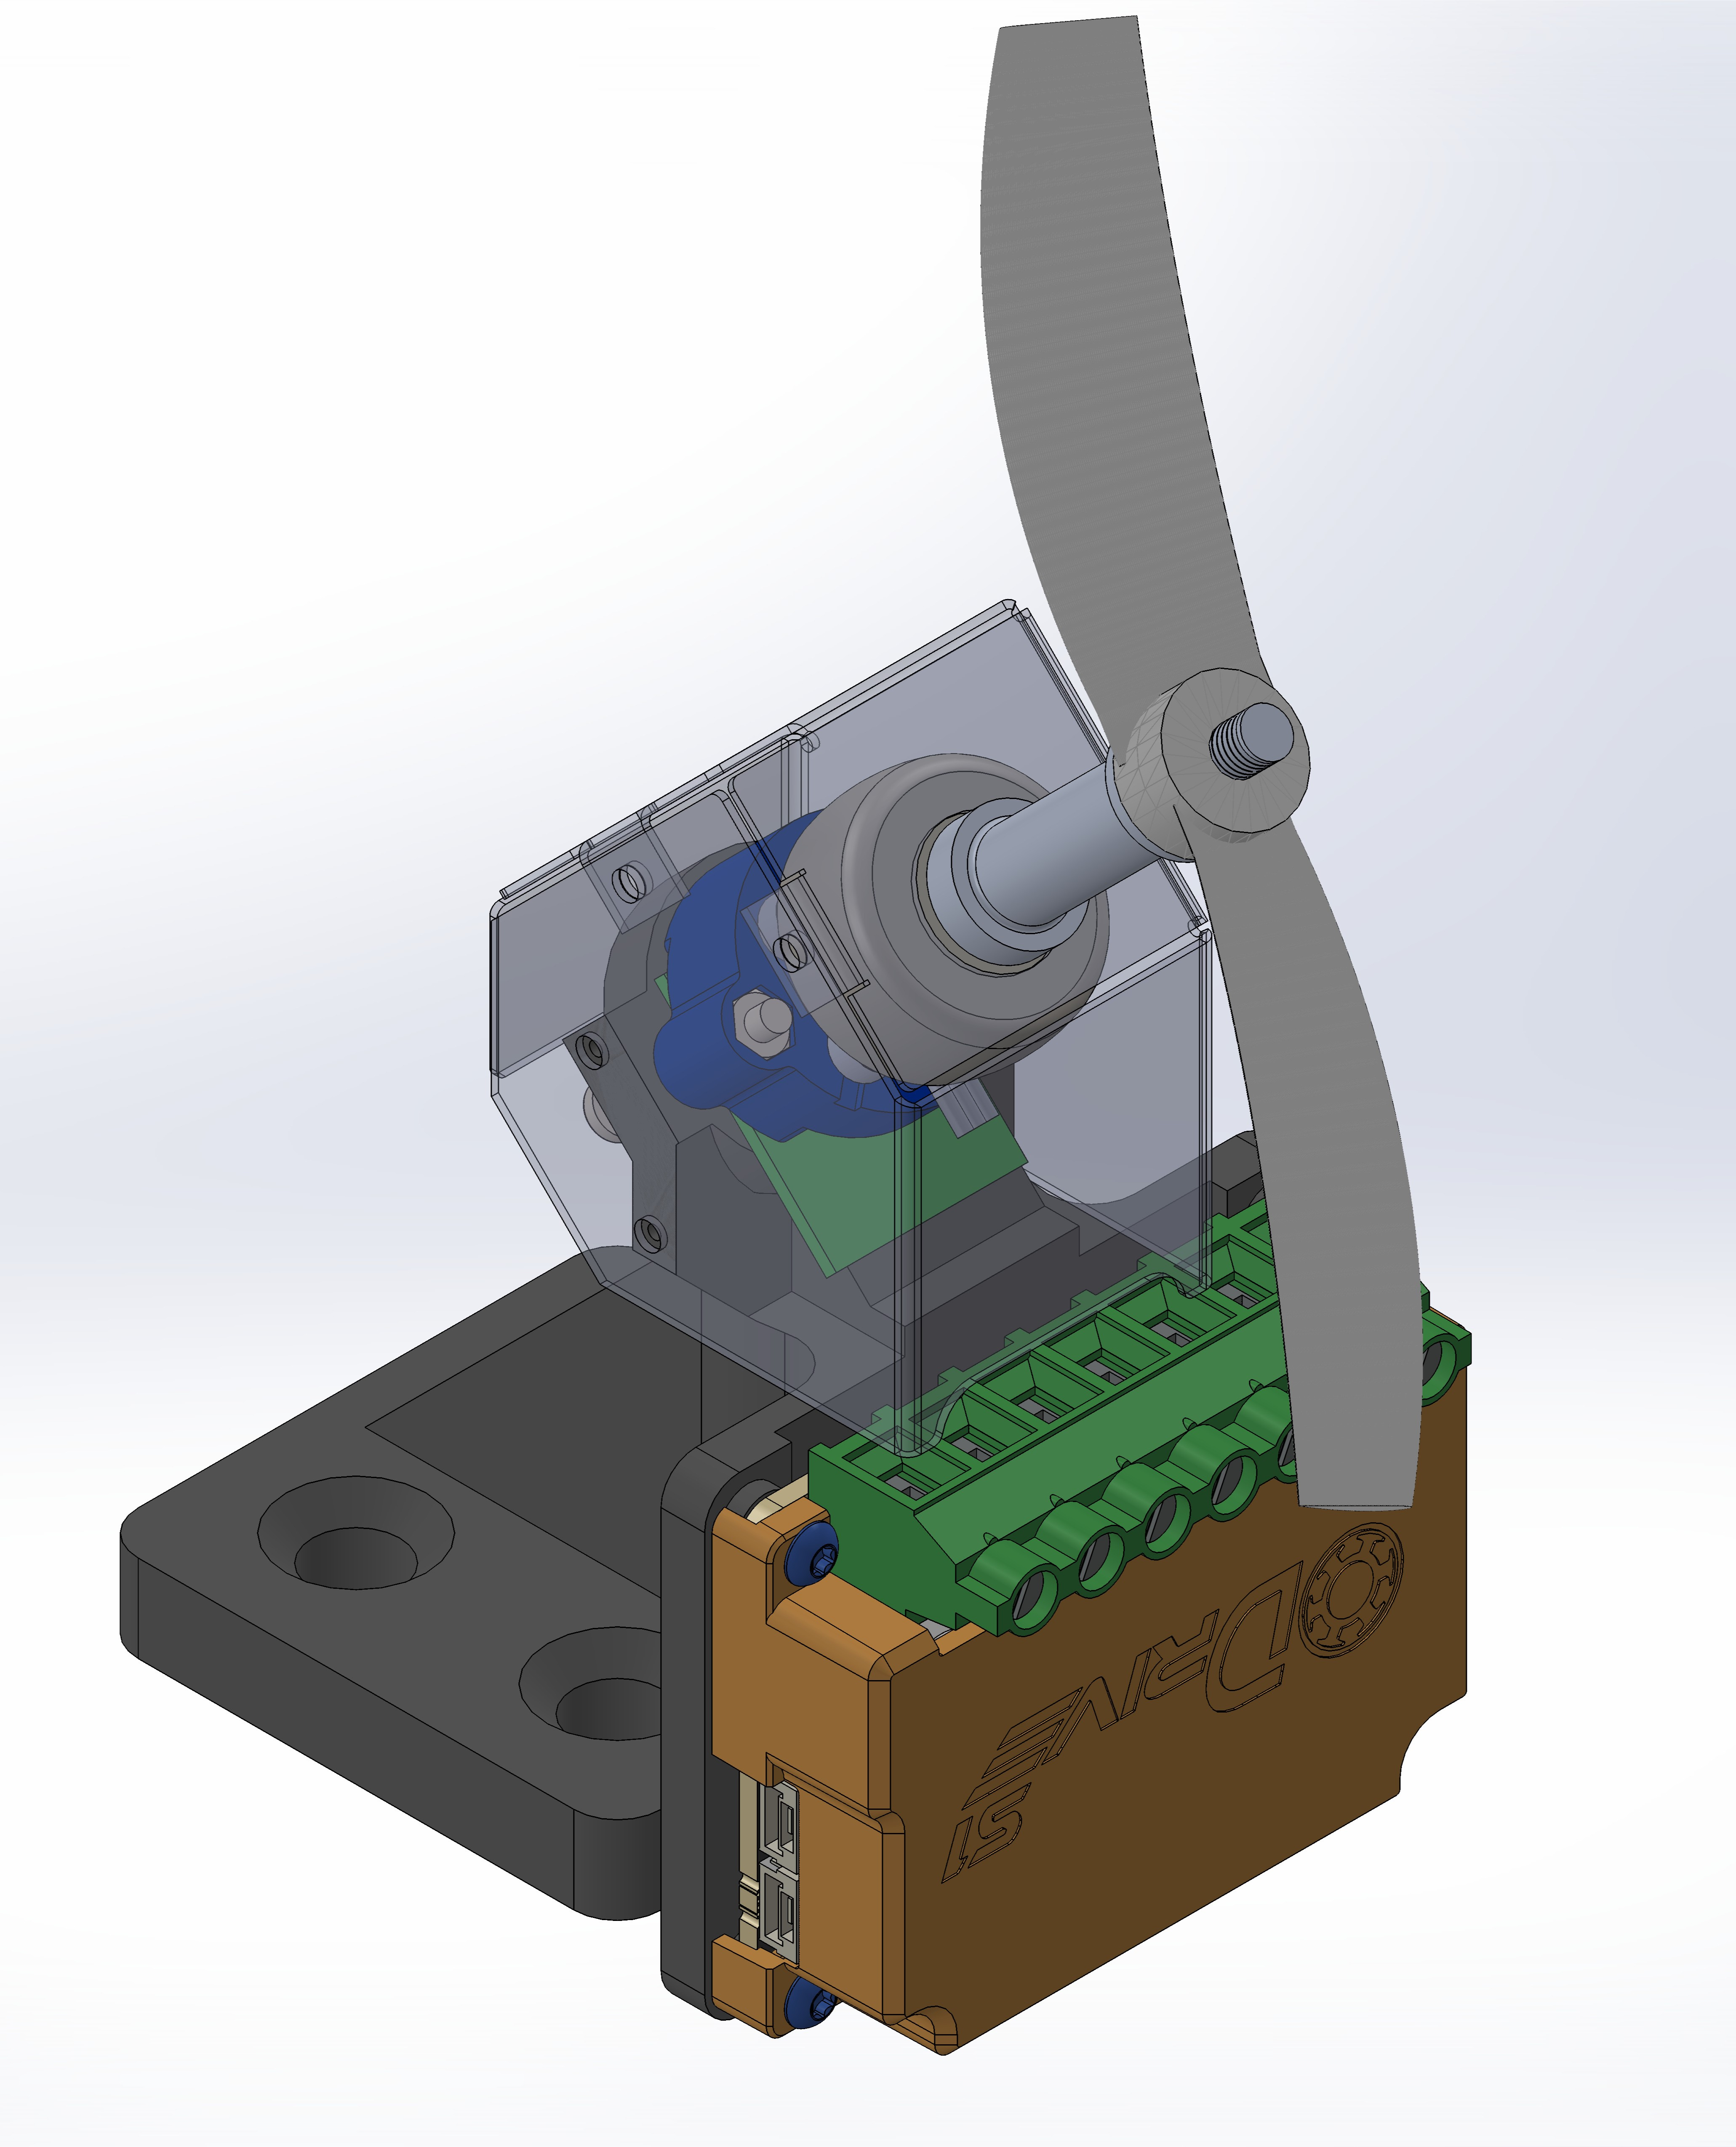
\includegraphics[height=5cm]{figures/acoustic1.JPG}
        \caption{}
        \label{fig:acoustic1}    
    \end{subfigure}
    \hfill
    \begin{subfigure}[t]{0.60\textwidth}
        \centering
        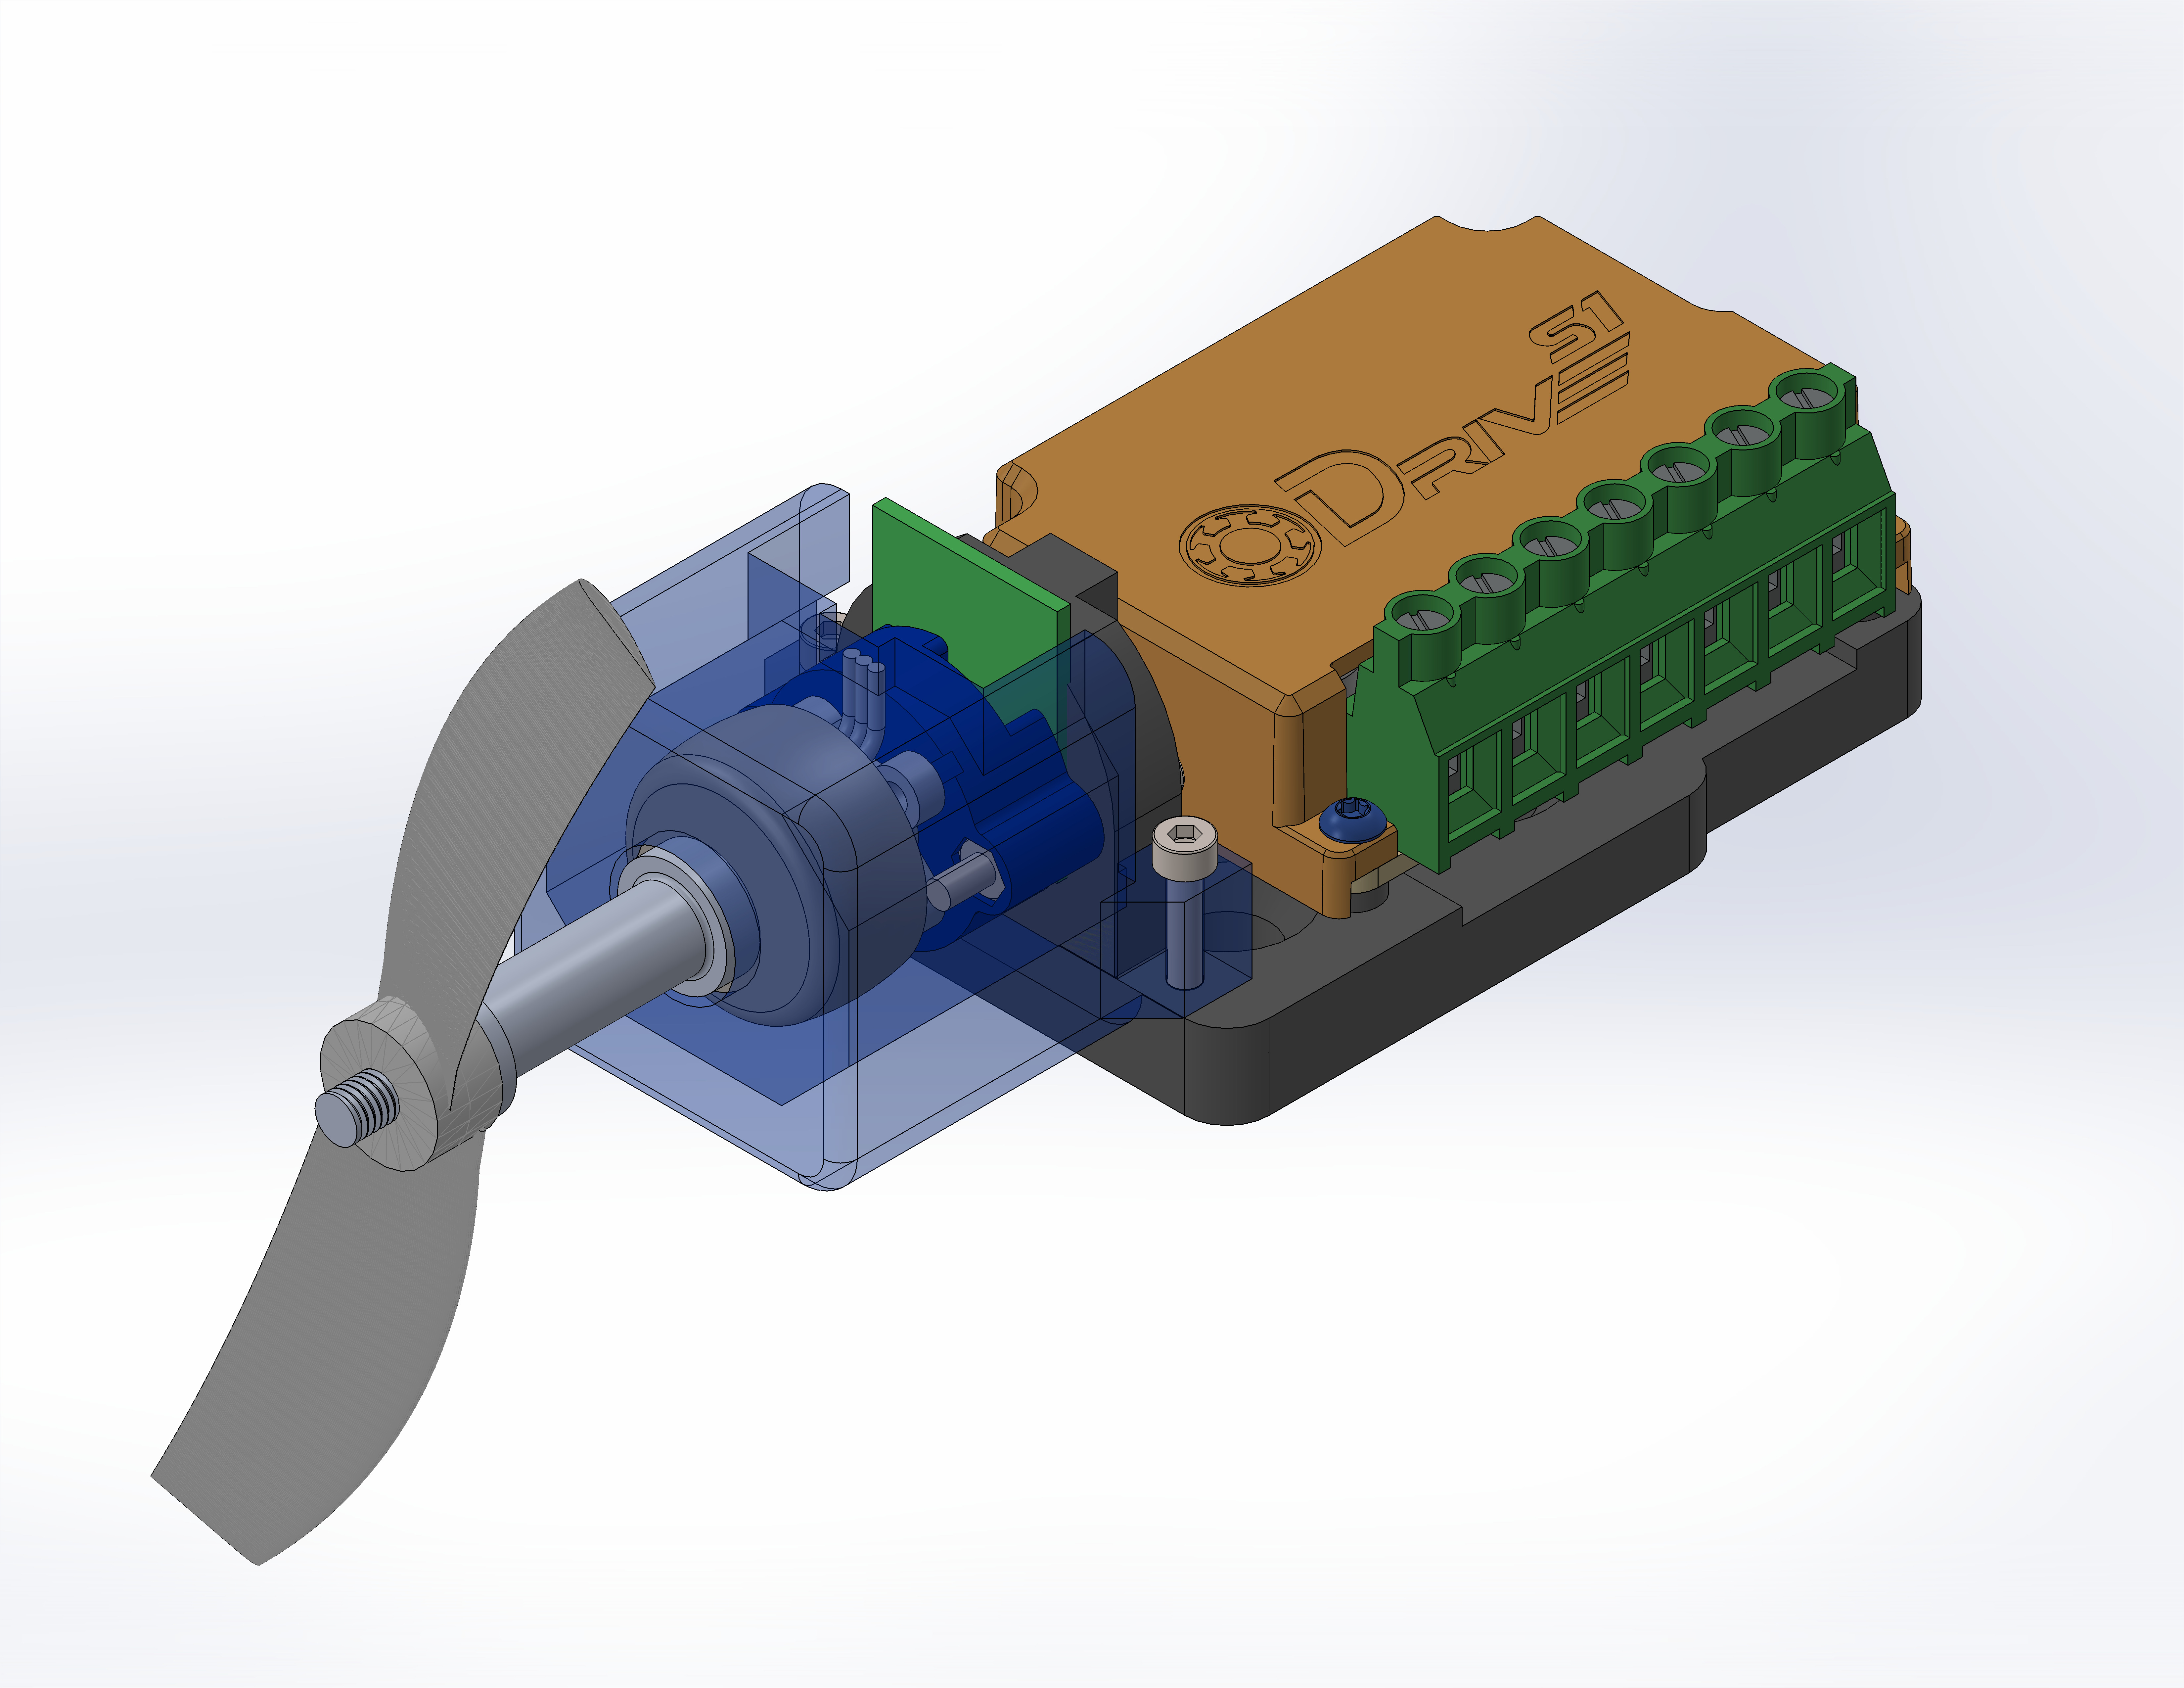
\includegraphics[height=6cm]{figures/acoustic2.JPG}
        \caption{}
        \label{fig:acoustic2}    
    \end{subfigure}
    \caption{Iterations of the acoustic test rig}
\end{figure}


\section{Key Experimental Challanges}

\subsection{Isolation of propeller noise}

As expected the motor noise is a significant source of interference with the propeller noise.
From vibration theory, the motor acts as a harmonic force input to the sprung mass stand.
This means that the rigid stand can be simply modelled as a 2nd order system.

Foam and rubber mounts were tested which had different damping and stiffness properties.
The sound spectrum of the motor only was measured for both mounts and can be compared.
TODO: consider analysing to justify the choice of mount.

\subsection{Comparison of with floor and without floor}
Another possible avenue



% key experimental parts to include
% tone generation
% concentricity
% Failed parts

\end{document}